\section{Experimental Evaluation}
\label{sec:exp}

In order to demonstrate the efficacy of our history-inclusion based
approximation to observational refinement, we argue that our $k$-approximation:
\begin{itemize}

  \item uncovers most violations with small values of $k$, and

  \item can be efficiently implemented, and vastly outperforms linearizability
  checking.

\end{itemize}

To argue both points, we have studied the concurrent data structure
implementations of Scal\footnote{Scal High-Performance Multicore-Scalable
Computing~\url{http://scal.cs.uni-salzburg.at}}, which include both LIFO- and
FIFO-based container objects. Some of these objects, such as the Michael-Scott
Queue~\cite{conf/podc/MichaelS96}, are meant to preserve observational
refinement\footnote{More precisely, they have been designed to be
linearizable.}, while others, such as Kirsch et al.'s
$k$-FIFO~\cite{conf/pact/KirschLP13}, are meant to preserve weaker properties.
For our experiments we have used Scal's C++ implementations without
modification, except to annotate methods with a fixed set of possible
preemption points, e.g.,~preceding accesses to shared storage.

To make the following comparisons, we have developed a tool for enumerating a
(large) number of alternate executions involving a limited number of object
method invocations. We execute each operation on a separate thread, and ensure
that all thread schedules up to a given number $n \in \<Nats>$ of thread
preemptions (at specified preemption points) are executed, similarly to
Microsoft's Chess tool~\cite{conf/osdi/MusuvathiQBBNN08}. With $n=0$
preemptions, there is only one schedule/execution, though the number of
schedules/executions grows exponentially as $n$ increases. For instance, with
our annotation of preemptions in Scal's Michael-Scott Queue, increasing
$n=1..5$ yields $33$, $612$, $8343$, $95434$, and $930141$ schedules, which are
executed at a rate of roughly one million schedules per minute on a MacBook Pro
2.6GHz Intel Core i5 machine.


\subsection{Coverage of Violations}

To show that most violations to observational refinement are uncovered by our
history inclusion approximation for small values of $k$, we have measured the
number of explored histories which are not linearizable, versus the number of
explored histories $h$ for which $A_k(h) |= \lnot @Y$. We use linearizability
as a metric for $h \in H(L)$, due to the equivalence of Section~\ref{sec:lin},
and since algorithms for computing linearizability are well
known~\cite{conf/pldi/BurckhardtDMT10}.

Figure~\ref{fig:data:coverage} shows that as the sample size of executions per
number of operations increases, number of violating histories $h$ for which
$A_k(h) |= \lnot @Y$ also increases. Furthermore, as the number of explored
histories increases beyond a certain point, the vast majority of violations $h$
are also detected by some explored $A_k(h') \preceq h$.

TODO DESCRIBE THIS BETTER AND MAKE IT CLEARER

\begin{figure}
  \centering
  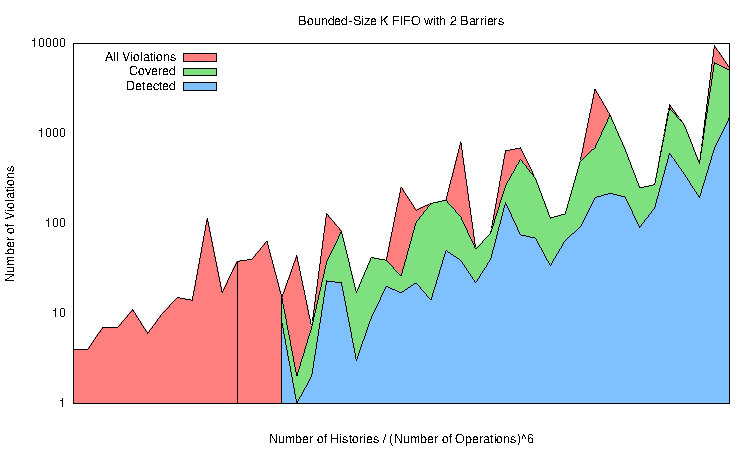
\includegraphics[width=\linewidth]{figures/coverage-bkq-2-barriers}
  \caption{Coverage of violations.}
  \label{fig:data:coverage}
\end{figure}

\subsection{Efficiency}

Figure~\ref{fig:data:runtime} compares the runtime of our operation-counting
instrumentation for $A_2$, versus a linearization-based instrumentation. The
x-axis shows the number of invoked operations, increasing from $2$ to $20$,
while the y-axis shows the total execution time of each approach on a
logarithmic scale, normalized to the total execution time without any
instrumentation. Though we have not specially optimized our implementation of
operation counting, we observe that runtime stays within the same order of
magnitude as without instrumentation. However, one clearly observes the cost
incurred by the exponential-time linearization algorithm: as the number of
operations increases --- and thus exponentially the number of possible
linearizations --- performance seriously degrades. With only $20$ operations,
instrumentation overhead is nearly $100,000$\%.


\begin{figure}
  \centering
  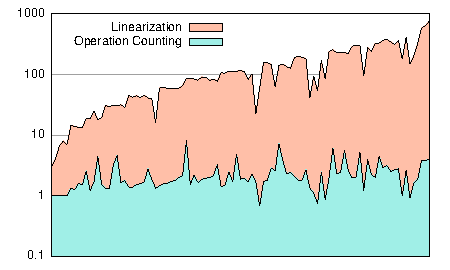
\includegraphics[width=\linewidth]{figures/lin-vs-counting-time}
  \caption{Runtime}
  \label{fig:data:runtime}
\end{figure}
